\documentclass{estilo}
\usepackage[spanish, es-tabla]{babel}
\usepackage{graphicx}
\usepackage{float}
\usepackage{amsmath}        % para los vectores columnas
\usepackage{amsfonts}       % para las negrita de pizarra
\usepackage{amssymb}        % para simbolos matematicos
\usepackage{hyperref}       % para utilizar referencias
\usepackage{multirow}       % para las tablas
\usepackage{booktabs}       % para tablas con estilo profesional e ingeniería
\usepackage{dsfont}
\usepackage{listings}
\usepackage{xcolor}
\usepackage{ragged2e}       % ¡CRÍTICO! Define el comando \justifying

\definecolor{codegreen}{rgb}{0,0.6,0}
\definecolor{codegray}{rgb}{0.5,0.5,0.5}
\definecolor{codepurple}{rgb}{0.58,0,0.82}
\definecolor{backcolour}{rgb}{0.95,0.95,0.92}

\lstdefinestyle{mystyle}{
    backgroundcolor=\color{backcolour},   
    commentstyle=\color{codegreen},
    keywordstyle=\color{magenta},
    numberstyle=\tiny\color{codegray},
    stringstyle=\color{codepurple},
    basicstyle=\ttfamily\footnotesize,
    breakatwhitespace=false,         
    breaklines=true,                  
    captionpos=b,                    
    keepspaces=true,                  
    numbers=left,                    
    numbersep=5pt,                  
    showspaces=false,                
    showstringspaces=false,
    showtabs=false,                  
    tabsize=2
}
\lstset{style=mystyle}

\usepackage{enumitem,multicol,setspace}
\newcounter{subenum}[enumi] % para las multicolumnas
\renewcommand{\thesubenum}{\arabic{subenum}}
\usepackage[nomessages]{fp}
\FPeval\thecolwidth{round(1/4:4)}% Specify number of columns -> column width
\newcommand{\newitem}[1]{%
  \refstepcounter{subenum}%
  \parbox{\dimexpr\thecolwidth\linewidth-.5\columnsep}{%
    \makebox[\labelwidth][r]{(\thesubenum)\hspace*{\labelsep}}%
    #1}\hfill%
}

\usepackage{scalerel,stackengine} % para el sombrero
\stackMath
\newcommand\rhat[1]{%
\savestack{\tmpbox}{\stretchto{%
  \scaleto{%
    \scalerel*[\widthof{\ensuremath{#1}}]{\kern-.6pt\bigwedge\kern-.6pt}%
    {\rule[-\textheight/2]{1ex}{\textheight}}%WIDTH-LIMITED BIG WEDGE
  }{\textheight}% 
}{0.5ex}}%
\stackon[1pt]{#1}{\tmpbox}%
}
\parskip 1ex

\usepackage{mathtools}      % floor y ceil
\DeclarePairedDelimiter\ceil{\lceil}{\rceil}
\DeclarePairedDelimiter\floor{\lfloor}{\rfloor} 

\usepackage[style=numeric, sorting=none]{biblatex}
\addbibresource{referencias.bib} % Archivo de bibliografía obligatorio

% --- Definición de parámetros para \maketitle (Exigido por estilo.cls) ---
\title{Propuesta de Trabajo Profesional: ParkLink \\ \vspace{0.2cm} \Large Sistema Integral de Mapeo, Gestión y Reserva de Cocheras Urbanas}
\author{Integrantes: [Alumno 1], [Alumno 2] \\ Tutor: [Nombre del Tutor] \\ Jefe de Cátedra: Mg. Ing. Carlos Fontela}
\date{\the\year}

\begin{document}

% --- Renderizado de la Carátula de la Cátedra ---
\maketitle 

\newpage
\justifying


\newpage
\tableofcontents

\newpage
% --- Cuerpo del Anteproyecto ---
\section{Resumen}
En las grandes ciudades, la disponibilidad de espacios de estacionamiento representa una problemática creciente debido al aumento del parque automotor y la limitada infraestructura urbana, generando congestión vehicular y dificultades para los conductores.

En este contexto, el presente proyecto propone el desarrollo de \textit{ParkLink}, una plataforma digital orientada a facilitar la búsqueda, publicación y reserva de espacios de estacionamiento, dirigida tanto a conductores como a propietarios de cocheras privadas y playas de estacionamiento.

La plataforma permitirá visualizar espacios disponibles mediante geolocalización, realizar reservas y gestionar publicaciones desde una única aplicación, incorporando autenticación de usuarios y procesamiento de pagos digitales.

En este trabajo desarrollaremos un Producto Mínimo Viable (MVP) que abarca los aspectos funcionales, técnicos y económicos del sistema, postergando integraciones avanzadas como sensores IoT o predicción con IA para fases posteriores.

\vspace{0.5cm}
\textbf{Palabras clave:} estacionamiento urbano, reserva de cocheras, geolocalización, plataforma digital, movilidad urbana.
\section{Abstract}
In large cities, finding a parking space is an everyday problem. The steady growth of the vehicle fleet and the limited urban infrastructure mean that a significant share of traffic consists of vehicles circulating without a concrete destination in search of a free spot, increasing congestion, fuel consumption and polluting emissions. At the same time, a large number of private garages and parking lots remain empty for much of the day due to the lack of a channel that reliably connects them with demand.

This Capstone Project documents the design, development and implementation of \textit{ParkLink}, a digital platform that connects drivers who need to park with owners of private garages and parking lots, using the Autonomous City of Buenos Aires (CABA) as its initial case study. The solution consists of a mobile application for Android and iOS, with differentiated experiences for drivers and owners, and a web administration panel intended for the platform's staff. Drivers can search for parking spaces on a georeferenced map, check their real availability, book them by the hour or for longer stays, and pay from within the application. Owners, in turn, publish their spaces, set prices, schedules and capacity, approve incoming requests and receive the settlement of their earnings. The system also includes in-person check-in verification through codes, messaging and support tied to each booking, user reviews, push and real-time notifications, refund management and listing moderation.

From a technical standpoint, the platform was built on an architecture of independent microservices, each with its own database, accessed through a single API gateway responsible for validating authentication through JWT tokens and routing requests. The mobile application and the administration panel were developed with React Native and Expo. The backend follows a polyglot approach: Python with FastAPI for the gateway, authentication and notifications; Go for booking and availability management; NestJS with TypeScript for parking space management; and Node.js with Express for payments. Persistence relies on PostgreSQL, using the PostGIS extension for proximity-based geographic searches, and asynchronous communication between services is based on events published over RabbitMQ. External services were also integrated for payment processing (Mercado Pago), push notifications (Firebase Cloud Messaging), email and SMS verification (Brevo and Twilio), image storage (Cloudflare R2) and error monitoring (Sentry), with all components containerized using Docker.

Development was managed with a hybrid agile methodology based on Scrum and Kanban practices, organized into fixed-length iterations with planning and story-point estimation, and supported by periodic meetings with the tutors to validate each increment. The source code was organized in a GitHub organization with an independent repository per microservice, integrated into a root repository through submodules, with code review through pull requests and continuous integration with GitHub Actions running static analysis and automated tests.

As a result, a functional Minimum Viable Product (MVP) was obtained that validates the technical and operational feasibility of the proposal, leaving more complex integrations
 for later stages. ParkLink thus helps reduce parking search time and unnecessary circulation, and promotes a more efficient use of existing urban infrastructure.

\section{Introducción}
La movilidad urbana representa uno de los principales desafíos de las grandes ciudades modernas. El crecimiento sostenido del parque automotor, combinado con la alta densidad poblacional y comercial de los centros urbanos, genera diariamente problemas vinculados con la congestión vehicular, la circulación ineficiente y la dificultad para acceder a espacios de estacionamiento disponibles. En ciudades como la Ciudad Autónoma de Buenos Aires (CABA), una parte considerable del tránsito diario está asociada a conductores que recorren múltiples cuadras buscando estacionamiento, incrementando no solo los tiempos de traslado, sino también el consumo de combustible, la contaminación ambiental y el nivel de estrés urbano.

Paralelamente, existe una gran cantidad de espacios de estacionamiento privados que permanecen desocupados durante extensos períodos de tiempo. Cocheras residenciales, estacionamientos comerciales y espacios pertenecientes a empresas u organizaciones suelen encontrarse subutilizados debido a la falta de herramientas que permitan conectarlos de manera eficiente con potenciales usuarios. Esta situación evidencia una ineficiencia en la distribución y utilización de recursos urbanos ya existentes.

A partir de esta problemática surge ParkLink, una plataforma digital orientada a facilitar la conexión entre conductores que necesitan estacionamiento y propietarios de espacios disponibles que desean monetizar su capacidad ociosa. El objetivo principal del proyecto es centralizar la oferta de estacionamiento mediante una aplicación accesible y sencilla, permitiendo visualizar espacios disponibles en tiempo real, realizar reservas y gestionar pagos de forma segura.

El proyecto se plantea inicialmente sobre un alcance acotado y escalable, priorizando el desarrollo de un Producto Mínimo Viable (MVP) que permita validar la utilidad y viabilidad del sistema en un entorno real. En esta primera etapa se busca desarrollar una solución funcional basada principalmente en reservas manuales y geolocalización, evitando incorporar tecnologías de automatización más complejas —como sistemas inteligentes de detección y predicción vehicular— que podrían incrementar significativamente los costos y riesgos de implementación.

Asimismo, ParkLink no solo busca brindar beneficios a los conductores, reduciendo tiempos de búsqueda y mejorando la experiencia de estacionamiento, sino también generar nuevas oportunidades económicas para propietarios de espacios subutilizados. De esta manera, el proyecto propone un modelo colaborativo que favorece una utilización más eficiente de la infraestructura urbana existente y contribuye al desarrollo de soluciones de movilidad más sostenibles para las grandes ciudades.

Finalmente, el desarrollo del sistema será llevado a cabo mediante una metodología híbrida basada en prácticas ágiles de Scrum y Kanban, permitiendo organizar el trabajo de manera iterativa, adaptable y orientada a la entrega progresiva de funcionalidades.

La definición del proyecto fue resultado de un proceso de generación de ideas y selección entre múltiples alternativas, cuyo análisis detallado se encuentra desarrollado en el \textbf{Anexo 1}.
\section{Estado del Arte y Mercado Potencial}

En los últimos años, el crecimiento sostenido de las grandes ciudades y el aumento del parque automotor impulsaron el desarrollo de múltiples soluciones tecnológicas orientadas a mejorar la movilidad urbana y asistir a los conductores durante sus desplazamientos. Dentro de este contexto, surgieron aplicaciones de navegación, sistemas de monitoreo de tránsito en tiempo real y plataformas de estacionamiento medido administradas por organismos municipales. Estas herramientas permiten optimizar recorridos, visualizar congestiones vehiculares y gestionar pagos asociados al uso del espacio público.

Sin embargo, gran parte de las soluciones actualmente disponibles se encuentran enfocadas principalmente en la circulación sobre la vía pública y en la administración de estacionamiento urbano regulado, dejando parcialmente desatendida la problemática relacionada con la disponibilidad, reserva y utilización eficiente de espacios privados de estacionamiento. En consecuencia, continúa existiendo una fragmentación significativa entre la oferta de cocheras privadas y la demanda de conductores que necesitan acceder rápidamente a un lugar seguro y cercano para estacionar.

A su vez, la creciente digitalización de servicios y la consolidación de modelos basados en economías colaborativas han demostrado la viabilidad de plataformas que permiten conectar usuarios con recursos ociosos mediante aplicaciones móviles y sistemas centralizados. Este paradigma abrió nuevas oportunidades para optimizar infraestructuras ya existentes sin necesidad de realizar grandes inversiones físicas adicionales.

En este escenario, ParkLink busca posicionarse como una plataforma capaz de integrar y centralizar distintos tipos de espacios de estacionamiento, permitiendo a conductores acceder a información unificada, realizar reservas anticipadas y gestionar pagos de manera digital y segura. El proyecto apunta especialmente a cubrir la falta de soluciones flexibles orientadas a reservas de corta duración y disponibilidad dinámica.

A nivel de mercado y competencia, pueden identificarse distintos modelos existentes que presentan limitaciones parciales frente a la propuesta planteada:

\begin{itemize}
\item \textbf{Estacionamiento libre y playas públicas:} representan la alternativa más tradicional utilizada por conductores urbanos. Sin embargo, su disponibilidad depende completamente de la ocupación inmediata, generando incertidumbre, tiempos prolongados de búsqueda y una fuerte variabilidad de precios según la zona y el horario.


\item \textbf{Sistemas de estacionamiento medido:} se encuentran limitados exclusivamente al uso de espacios públicos sobre la vía urbana. Generalmente no permiten reservas anticipadas y operan bajo restricciones horarias y regulatorias definidas por cada municipio.

\item \textbf{Plataformas de alquiler de cocheras tradicionales:} suelen estar orientadas a contratos mensuales o de larga duración, priorizando usuarios permanentes por sobre necesidades temporales o transaccionales. Esto reduce considerablemente la flexibilidad para conductores que requieren estacionamiento únicamente por horas o períodos breves.

\item \textbf{Aplicaciones de navegación y tráfico:} herramientas como sistemas GPS o plataformas de mapas colaborativos brindan información sobre tránsito y rutas, pero no ofrecen integración completa con reservas de estacionamiento privado ni mecanismos centralizados de contratación.


\end{itemize}

A partir de este análisis, se observa una oportunidad concreta para el desarrollo de una plataforma que combine geolocalización, reserva anticipada, gestión digital de pagos y utilización colaborativa de espacios subutilizados. De esta manera, ParkLink busca diferenciarse mediante un enfoque centrado en la flexibilidad, accesibilidad y optimización de recursos urbanos existentes, apuntando inicialmente a contextos urbanos de alta densidad como la Ciudad Autónoma de Buenos Aires.

\section{Análisis de Negocio}\label{sec:negocio}

Con el objetivo de validar la viabilidad estratégica de ParkLink y establecer un marco claro para la toma de decisiones, se aplicaron dos herramientas de análisis de negocios ampliamente utilizadas en la industria: El modelo de las 5C's, que permite mapear el entorno competitivo y colaborativo del proyecto, y el esquema de las 4P's, que estructura la propuesta de valor desde una perspectiva de marketing y posicionamiento.

\subsection{Análisis de las 5C's}

\subsubsection{Compañía (\textit{Company})}

ParkLink es una plataforma web y móvil que actúa como marketplace transaccional de estacionamiento urbano. Su propuesta de valor central consiste en conectar a conductores que necesitan un lugar donde estacionar con propietarios de espacios ociosos o cocheras comerciales, facilitando la reserva anticipada, la gestión de disponibilidad y el pago digital en un único entorno unificado.

La estructura del sistema se organiza en cuatro módulos de trabajo independientes (mapeo y geolocalización, reserva dinámica, autenticación y seguridad, y pagos), cuyo detalle técnico se desarrolla en la sección de Metodología. Este enfoque modular permite un desarrollo incremental alineado con los recursos disponibles del equipo.

La detección automática de disponibilidad mediante sensores IoT, predicciones mediante sistemas de IA y la integración con sistemas municipales de tránsito se identifican como evoluciones futuras fuera del alcance del MVP, dada la complejidad técnica y los recursos externos que requieren.

El principal riesgo operativo del modelo es el problema del arranque en frío: Para que la plataforma funcione, se necesitan simultáneamente propietarios que ofrezcan espacios y conductores que los demanden. La estrategia para mitigar esto consiste en lanzar en una zona geográfica acotada de CABA, donde sea posible generar masa crítica en ambos lados del mercado antes de escalar.

\subsubsection{Clientes y Segmentación (\textit{Customers})}

ParkLink atiende a cuatro segmentos de usuarios con necesidades diferenciadas:

\begin{enumerate}
    \item \textbf{Conductores particulares:} Representan el lado de la demanda. Su necesidad principal es encontrar un espacio disponible, con precio conocido de antemano, sin necesidad de circular en busca de lugar. Es el segmento más fácil de captar inicialmente porque comprende el valor del producto de forma inmediata.

    \item \textbf{Propietarios de espacios privados:} Personas con cocheras o entradas de garaje que permanecen vacías durante determinados períodos del día. Su motivación es generar ingresos pasivos a partir de un activo subutilizado, sin necesidad de gestión adicional.

    \item \textbf{Playas y cocheras comerciales:} Estacionamientos que buscan incrementar su tasa de ocupación mediante reservas anticipadas y captación de usuarios a través de un canal digital. Aportan mayor volumen de oferta y pueden acceder a herramientas de gestión de tarifas y disponibilidad.

    \item \textbf{Flotas, empresas y conductores frecuentes:} Repartidores, técnicos de campo, vehículos corporativos que necesitan previsibilidad en el estacionamiento. Representan un segmento con alta recurrencia y potencial para planes de suscripción mensual.
\end{enumerate}

Un quinto segmento de interés es el \textbf{municipio o actores públicos}, que podrían convertirse en clientes institucionales en una etapa posterior, una vez que la plataforma demuestre capacidad para gestionar datos de movilidad urbana a escala. Este segmento queda fuera del alcance del MVP por los largos procesos de licitación y los requisitos técnicos y legales que implica.

En términos de modelo de cobro, se definió que el único pagador fuera el conductor, mediante un cargo de servicio sobre cada reserva concretada, y que el propietario no tuviera ningún costo por publicar ni por cada operación. De esta forma se evita cobrar al lado de la oferta, que es el más difícil de captar en las primeras etapas de un mercado de dos lados.

\subsubsection{Competidores (\textit{Competitors})}

El análisis detallado de los competidores —incluyendo sus ventajas y limitaciones frente a ParkLink— se desarrolla en la Sección~\ref{sec:estado_arte}. A modo de síntesis, los actores relevantes son: El estacionamiento libre en la vía pública, los sistemas de estacionamiento medido (Blinkay), los navegadores con información de tráfico (Waze, Google Maps), los clasificados digitales (MercadoLibre, OLX) y las plataformas internacionales de referencia (SpotHero, EasyPark). Ninguno de los actores locales cubre de forma integral la intersección entre reserva anticipada, disponibilidad en tiempo real, pago digital y acceso a espacios privados que define la propuesta de ParkLink.

\subsubsection{Colaboradores (\textit{Collaborators})}

Para conseguir un mayor volumen de clientes, ParkLink deberá valerse de diversas alianzas estratégicas con actores clave del ecosistema de movilidad urbana y gestión de espacios en grandes ciudades:

\begin{itemize}
    \item \textbf{Propietarios y administradores de cocheras:} Su disposición a incorporarse a la plataforma define el tamaño de la oferta disponible.
    \item \textbf{Usuarios de la plataforma:} Su experiencia y satisfacción determinarán la tasa de retención y el crecimiento orgánico a través de recomendaciones.
    \item \textbf{Administradores de edificios:} Canal natural de acceso a propietarios de cocheras residenciales en zonas de alta densidad.
    \item \textbf{Municipalidades:} Fuente de información sobre regulaciones, zonas de estacionamiento medido y potenciales alianzas a futuro.
\end{itemize}

\subsubsection{Contexto del Entorno (\textit{Context})}

El entorno en el que ParkLink se desarrolla presenta condiciones favorables para su adopción:

\begin{itemize}
    \item \textbf{Social:} La población urbana ya utiliza con normalidad aplicaciones de mapas, reservas y pagos digitales. La adopción de plataformas de economía colaborativa estableció patrones de comportamiento compatibles con el modelo de ParkLink.
    \item \textbf{Tecnológico:} La penetración de smartphones en Argentina supera el 80\%, y la conectividad móvil en zonas urbanas permite el uso fluido de aplicaciones con geolocalización en tiempo real.
    \item \textbf{Económico:} En contextos de inflación, la monetización de activos ociosos como cocheras resulta especialmente atractiva para propietarios. Para conductores, conocer el precio exacto antes de llegar reduce la incertidumbre económica del traslado.
    \item \textbf{Legal y Regulatorio:} El uso de espacios privados como cocheras para alquiler temporal tiene respaldo en el Código Civil y Comercial, bajo la figura de la locación. El tratamiento de datos personales está regulado por la Ley 25.326 y la normativa de la AAIP, detalladas en el \hyperref[anexo:legal]{Anexo 3}.
\end{itemize}

\subsection{Análisis de las 4P's}

\subsubsection{Producto (\textit{Product})}

ParkLink es una aplicación móvil y plataforma web que permite encontrar, reservar y pagar espacios de estacionamiento en la Ciudad Autónoma de Buenos Aires.

El sistema contempla tres experiencias de usuario diferenciadas:

\begin{itemize}
    \item \textbf{Experiencia del conductor:} Accede a un mapa interactivo con los espacios disponibles cercanos, visualiza el precio y el horario de disponibilidad de cada uno, realiza una reserva indicando la duración estimada, y llega directamente al espacio confirmado sin necesidad de circular en busca de lugar.
    \item \textbf{Experiencia del propietario particular:} Publica su cochera o espacio libre, define los horarios en que está disponible y el precio por hora, y recibe reservas de forma automática sin necesidad de intervención adicional por cada operación.
    \item \textbf{Experiencia de playas comerciales:} Gestiona su capacidad disponible, establece tarifas diferenciadas por horario o tipo de vehículo, y recibe reservas anticipadas que le permiten optimizar la ocupación de sus instalaciones.
\end{itemize}

El diferencial competitivo central frente a los actores locales existentes es la combinación de reserva anticipada con confirmación de disponibilidad real, pago integrado y acceso a espacios privados. A diferencia de Blinkay, que informa sobre el estacionamiento medido pero no permite reservar; y a diferencia de los clasificados digitales, que facilitan alquileres mensuales pero no transacciones por horas, ParkLink resuelve el problema completo del conductor en una única interfaz.

\subsubsection{Precio (\textit{Price})}

ParkLink no cobra a los propietarios: El ingreso de la plataforma proviene exclusivamente de las transacciones exitosas y lo abona únicamente el conductor. El modelo de ingresos se estructura de la siguiente forma:

\begin{itemize}
    \item \textbf{Propietario:} Publica su cochera sin costo y recibe el 100\% del precio que fija para su espacio.
    \item \textbf{Cargo de servicio al conductor:} 8\% adicional sobre el valor de cada reserva concretada, abonado por el conductor al momento del pago como cargo de plataforma.
\end{itemize}

Este esquema garantiza que publicar sea gratuito para los propietarios y que reciban la totalidad de su tarifa, eliminando barreras de entrada al lado de la oferta. Al mismo tiempo, alinea los incentivos de la plataforma con el éxito de cada operación: ParkLink solo genera ingresos cuando hay una transacción real.

Para etapas posteriores se contempla la posibilidad de incorporar planes de suscripción mensual para cocheras comerciales con alto volumen de reservas, servicios de visibilidad destacada en el mapa, y planes para flotas empresariales con tarifas negociadas y facturación centralizada.

\subsubsection{Plaza (\textit{Place})}

La distribución de ParkLink es 100\% digital. El acceso a la plataforma se realiza a través de:

\begin{itemize}
    \item Aplicación móvil multiplataforma para iOS y Android.
    \item Plataforma web accesible desde cualquier dispositivo con navegador.
\end{itemize}

La estrategia de lanzamiento contempla un despliegue geográfico progresivo:

\begin{enumerate}
    \item \textbf{MVP (año 1):} Foco en barrios de CABA con alta densidad vehicular y demanda de estacionamiento comprobada (Palermo, Recoleta y microcentro). El objetivo es generar masa crítica local antes de escalar.
    \item \textbf{Mediano plazo (año 2):} Expansión a toda la Ciudad Autónoma de Buenos Aires y primeros municipios del Gran Buenos Aires.
    \item \textbf{Largo plazo:} Expansión a otras ciudades argentinas de alta densidad (Córdoba, Rosario, Mendoza) y evaluación de mercados de América Latina.
\end{enumerate}

\subsubsection{Promoción (\textit{Promotion})}

La estrategia de adquisición de usuarios se diferencia según el segmento objetivo:

\paragraph{Estrategia de demanda (conductores):}
\begin{itemize}
    \item Campañas en Google Ads segmentadas por búsquedas relacionadas con estacionamiento en CABA.
    \item Publicidad geolocalizada en Instagram y TikTok orientada a conductores en zonas de alta congestión.
    \item Presencia en comunidades de conductores y grupos de afinidad automotriz en redes sociales.
\end{itemize}

\paragraph{Estrategia de oferta (propietarios):}
\begin{itemize}
    \item Contacto directo con administradores de edificios de alta densidad en las zonas de lanzamiento.
    \item Campañas en redes sociales orientadas a propietarios de inmuebles en CABA.
    \item Comunicación enfocada en el ingreso pasivo: «Tu cochera vacía puede generar ingresos mientras no la usás».
\end{itemize}

\paragraph{Tácticas de crecimiento orgánico y referidos:}
\begin{itemize}
    \item Programa de referidos entre propietarios: Visibilidad destacada en el mapa por cada nuevo espacio incorporado a través de una recomendación.
    \item Visibilidad destacada en el mapa para los primeros propietarios en cada nueva zona de expansión, como incentivo de adopción temprana.
    \item Generación de contenido sobre movilidad urbana y estacionamiento en CABA, posicionando a ParkLink como referente del tema en medios digitales.
\end{itemize}

\section{Problema detectado y/o faltante}\label{sec:problema}

La creciente densidad vehicular en los grandes centros urbanos ha evidenciado múltiples limitaciones en la manera en que actualmente se gestionan y utilizan los espacios de estacionamiento. A pesar de la existencia de cocheras privadas, estacionamientos comerciales y sistemas de estacionamiento medido, persiste una importante falta de integración tecnológica que permita conectar de manera eficiente la oferta disponible con la demanda de los conductores.

En ciudades de alta circulación como la Ciudad Autónoma de Buenos Aires, la búsqueda de estacionamiento representa una problemática cotidiana que impacta tanto en la movilidad urbana como en la experiencia de los usuarios. El problema no radica en la falta de opciones, sino en la falta de información: La oferta existe, pero el conductor no puede verla ni compararla en el momento en que debe decidir. Esta situación genera pérdidas de tiempo, circulación innecesaria y una utilización ineficiente de recursos urbanos ya existentes.

\subsection{Puntos críticos del problema}

A partir del análisis realizado, se identificaron los siguientes puntos críticos:

\begin{enumerate}
\item \textbf{Pérdida de tiempo y falta de previsibilidad:} Los conductores particulares no cuentan con mecanismos confiables que les permitan asegurar un espacio de estacionamiento antes de llegar a destino. Como consecuencia, gran parte del tiempo de circulación en zonas urbanas se destina a la búsqueda manual de lugares disponibles, generando demoras frecuentes, congestión vehicular y aumento en los costos operativos asociados al traslado.

\item \textbf{Subutilización de espacios privados:} Existe una cantidad considerable de cocheras residenciales, estacionamientos comerciales y espacios pertenecientes a empresas que permanecen desocupados durante determinados períodos del día. Sin embargo, muchos propietarios no disponen de una plataforma segura, simple y masiva que les permita ofrecer temporalmente dichos espacios a potenciales usuarios interesados.

\item \textbf{Fragmentación y falta de visibilidad de la oferta:} La oferta de estacionamiento se encuentra distribuida entre múltiples actores y canales independientes, sin un medio que permita conocer de antemano su disponibilidad, ubicación y precio. El conductor solo descubre cada opción cuando pasa frente a ella, por lo que no puede compararlas y termina decidiendo con información incompleta.

\item \textbf{Complejidad transaccional y falta de confianza:} La inexistencia de un sistema integrado que combine geolocalización, reservas digitales, validación de identidad y procesamiento seguro de pagos dificulta la adopción de modelos colaborativos de estacionamiento. Tanto conductores como propietarios suelen percibir incertidumbre respecto a la seguridad, confiabilidad y formalidad de este tipo de intercambios.

\item \textbf{Impacto urbano y ambiental:} La circulación innecesaria derivada de la búsqueda de estacionamiento incrementa la congestión vehicular, el consumo de combustible y la emisión de gases contaminantes. Esto no solo afecta la experiencia individual de los conductores, sino también la eficiencia general del sistema de movilidad urbana.
\end{enumerate}

\subsection{La búsqueda de estacionamiento como problema de parada óptima}

La dificultad de fondo que enfrenta el conductor tiene una formulación matemática precisa: Se trata de un \textbf{problema de parada óptima} (\textit{optimal stopping}). Esta familia de problemas, estudiada por la teoría de la probabilidad y la investigación operativa, describe situaciones en las que una persona evalúa opciones de a una por vez, en un orden que no controla, y debe decidir en cada momento si acepta la opción que tiene delante o la descarta para seguir buscando, sabiendo que una opción descartada no puede recuperarse. Su ejemplo más conocido es el llamado problema de la secretaria, en el que se debe elegir al mejor candidato de una serie de entrevistas sin poder volver a convocar a los rechazados \autocite{ferguson1989}. Su solución dio origen a la conocida regla del 37\%: Observar sin decidir durante aproximadamente el primer 37\% de la búsqueda y luego aceptar la primera opción que supere a todas las anteriores. Aun aplicando esta estrategia óptima, la probabilidad de elegir la mejor opción es de apenas un 37\% \autocite{christian2016}.

El estacionamiento cuenta con su propia versión de este problema, formulada por MacQueen y Miller \autocite{macqueen1960} y conocida como el \textbf{problema del estacionamiento} (\textit{parking problem}). En ella, un conductor avanza por una calle hacia su destino y quiere estacionar lo más cerca posible de él. A medida que avanza solo puede ver el lugar que tiene enfrente, sin saber si más adelante habrá uno libre, y una vez que deja pasar un lugar no puede volver a él. La estrategia óptima para este problema es de umbral: Ignorar los lugares disponibles hasta cierta distancia del destino y, a partir de allí, tomar el primero que esté libre. Esa distancia depende de cuán ocupada esté la calle; por ejemplo, si nueve de cada diez lugares están ocupados, conviene empezar a buscar seis lugares antes del destino \autocite{fergusonstopping}. Las variantes posteriores del problema, como la que permite dar la vuelta para regresar a un lugar ya visto a cambio de un costo adicional, confirman que la falta de información sobre lo que hay más adelante es la que obliga al conductor a decidir sin certezas \autocite{tamaki1988}.

Este marco permite entender por qué, en la mayoría de los casos, el conductor termina eligiendo mal, aun cuando existen buenas opciones disponibles. Lo mismo que ocurre con los lugares en la calle ocurre con las cocheras y las playas de estacionamiento: El conductor las descubre de a una, a medida que circula, sin conocer su precio ni su disponibilidad hasta llegar a cada una, y sin saber si a dos cuadras hay una alternativa más cercana o más económica. Ante la incertidumbre y el apuro, la decisión racional suele ser aceptar la primera opción aceptable. El problema, por lo tanto, no son las cocheras ni las playas comerciales, que constituyen una oferta valiosa y necesaria, sino la escasa visibilidad y la imposibilidad de comparar, que convierten cada búsqueda en una apuesta.

ParkLink ataca el problema en su raíz: En lugar de ayudar al conductor a elegir mejor dentro de una búsqueda secuencial, elimina la búsqueda secuencial. Al mostrar sobre un mismo mapa todas las opciones cercanas al destino, con su precio y su disponibilidad real, y permitir reservarlas antes de salir, transforma un problema de parada óptima con información incompleta en una elección simultánea con información completa, en la que el conductor puede comparar todas las alternativas y quedarse con la que mejor se ajusta a lo que necesita.

\subsection{Cuantificación del costo de la búsqueda}

Más allá de la incomodidad, buscar estacionamiento en Buenos Aires tiene un costo económico concreto y medible. Cada vez que un conductor sale sin saber dónde va a estacionar, está asumiendo una pérdida que pocas veces se percibe como tal porque aparece repartida en tiempo, combustible, riesgo y decisiones tomadas sin información.

\textbf{Tiempo perdido.} Se estima que un conductor urbano en CABA dedica aproximadamente 15 minutos por salida a dar vueltas buscando un lugar libre. Tomando como referencia el salario promedio de la Ciudad de Buenos Aires en 2026 --- aproximadamente \$2.216.804 ARS mensuales \autocite{infobae_salarios_2026} ---, esos 15 minutos equivalen a unos \$3.464 ARS en tiempo que simplemente no se recupera.

\textbf{Combustible.} Durante esa búsqueda el auto recorre entre 2 y 3 kilómetros en condiciones de tránsito urbano: Marcha lenta, frenadas constantes, el escenario de mayor consumo posible. Con un consumo estimado de 10 litros cada 100 km y el precio de la nafta premium en CABA a marzo de 2026 --- \$2.223 ARS por litro \autocite{economista_nafta_2026} ---, ese recorrido representa unos \$556 ARS en combustible por búsqueda.

\textbf{Riesgo de multa.} Cuando la búsqueda no termina bien y el conductor decide estacionar en un lugar indebido, el costo puede ser alto: La multa por estacionamiento indebido en CABA asciende a \$94.999 ARS \autocite{infobae_multas_2026}. Considerando que un conductor urbano promedio acumula una infracción de este tipo aproximadamente cada seis meses --- unas 120 salidas ---, el valor esperado de ese riesgo es de \$792 ARS por cada vez que se estaciona.

\textbf{Elegir sin poder comparar.} Cuando el tiempo apremia, el conductor termina aceptando la primera cochera o playa disponible, sin haber podido comparar precios con las alternativas cercanas, tal como predice el problema de parada óptima. En CABA, el precio de una hora de estacionamiento varía entre \$6.000 y \$10.000 ARS según la zona y el horario, y puede alcanzar los \$20.000 ARS en las zonas de mayor demanda \autocite{iprofesional2026cocheras}. Elegir a ciegas implica, por lo tanto, quedar expuesto a pagar el extremo alto de ese rango cuando a pocas cuadras había una opción más conveniente: En una estadía de dos horas, la diferencia entre ambos extremos alcanza los \$8.000 ARS. Si esto ocurre una vez cada diez salidas, el sobrecosto esperado por búsqueda es de unos \$800 ARS.

\begin{table}[H]
\centering
\renewcommand{\arraystretch}{1.5}
\resizebox{\textwidth}{!}{%
\begin{tabular}{|l|r|}
\hline
\textbf{Concepto} & \textbf{Costo estimado por búsqueda} \\
\hline
Tiempo perdido (\textasciitilde15 min) & \$3.464 ARS \\
Combustible (\textasciitilde0,25 L) & \$556 ARS \\
Riesgo de multa (1 cada 6 meses) & \$792 ARS \\
Sobrecosto por elegir sin comparar (1 cada 10 salidas) & \$800 ARS \\
\hline
\textbf{Total estimado} & \textbf{\$5.612 ARS} \\
\hline
\end{tabular}%
}
\caption{Costo estimado por evento de búsqueda de estacionamiento en CABA (2026)}
\label{tab:costo_insatisfaccion}
\end{table}

A estos valores se suman costos intangibles pero igualmente significativos: El impacto en la puntualidad, el estrés de la incertidumbre y la productividad perdida por quienes dependen de una llegada a tiempo. La suma de todos estos factores define el costo real de no tener garantizado un espacio de estacionamiento antes de salir.

Incluso, algunas grandes ciudades de América Latina implementaron medidas regulatorias para limitar la circulación vehicular debido a los altos niveles de congestión urbana. Un ejemplo de ello es el sistema conocido como ``Pico y Placa'', utilizado en ciudades como Bogotá y Medellín, en Colombia, donde la circulación de vehículos se restringe determinados días y horarios según el número final de la patente. Este tipo de políticas refleja la magnitud del problema asociado a la movilidad urbana y evidencia la necesidad de desarrollar soluciones tecnológicas complementarias que permitan optimizar el uso de la infraestructura existente, reducir la circulación innecesaria y mejorar la experiencia de los conductores.

En función de estas problemáticas, surgió la necesidad de desarrollar una solución tecnológica que permitiera centralizar la información, hacer visible toda la oferta disponible y simplificar la interacción entre conductores y propietarios. ParkLink se desarrolló para responder a esta necesidad mediante una plataforma digital que permite comparar y reservar estacionamiento antes de salir, reduce la incertidumbre del conductor y promueve una utilización más eficiente de la infraestructura urbana existente.

\section{Solución Propuesta}
Se propone el desarrollo de una plataforma web y móvil integral que actúe como un ecosistema transaccional y de geolocalización. Para asegurar la factibilidad técnica y respetar las restricciones de recursos humanos y temporales de la carrera, el alcance del Producto Mínimo Viable (MVP) se estructurará de forma modular, priorizando la carga manual y la reserva programada.

\subsection{División en Módulos de Trabajo}
\begin{itemize}
    \item \textbf{Módulo de Mapeo y Geolocalización:} Visualización de plazas disponibles sobre mapas digitales interactivos mediante la integración de APIs de cartografía.
    \item \textbf{Módulo de Reserva Dinámica:} Motor lógico para la gestión de disponibilidad horaria y reservas manuales en tiempo real.
    \item \textbf{Módulo de Autenticación y Seguridad:} Gestión de perfiles diferenciados para conductores (demandantes) y propietarios/playas (oferentes).
    \item \textbf{Módulo de Pagos:} Integración con procesadores de pago y billeteras virtuales para la retención automática de comisiones y liquidación a proveedores.
\end{itemize}

\subsection{Nota sobre el Alcance y Restricciones}
Si bien la visión a largo plazo contempla la integración de sensores IoT para la detección automática de ocupación física en tiempo real y componentes de Inteligencia Artificial descriptiva para predicción de demanda, se concluye que dichos elementos representan un riesgo de complejidad elevado para la fase inicial. Por lo tanto, se posponen como evoluciones futuras del sistema.
\section{Diseño y Arquitectura de Software}

Se optó por una arquitectura cliente-servidor con microservicios. Este enfoque permite separar las funcionalidades por dominio, escalar cada servicio según su carga particular y desplegar cambios sin afectar al resto del sistema.

\subsection{Aplicación móvil}
\textbf{React Native} \autocite{reactnative}. Es el canal principal de uso para conductores y propietarios. Se eligió React Native para soportar iOS y Android con una sola base de código.

\subsection{Microservicios}
\textbf{Node.js} \autocite{nodejs} con \textbf{TypeScript} \autocite{typescript}. Implementan la lógica de negocio del sistema y exponen las APIs REST que consume la app móvil.

\subsection{Base de datos}
\textbf{PostgreSQL} \autocite{postgresql} con la extensión \textbf{PostGIS} \autocite{postgis}. Persiste los datos del sistema (usuarios, cocheras, reservas, pagos). PostGIS habilita las búsquedas de cocheras por proximidad geográfica.

\subsection{Caché}
\textbf{Redis} \autocite{redis}. Acelera el acceso a datos consultados frecuentemente: sesiones de usuario, tokens y disponibilidad de cocheras en tiempo real.

\subsection{Mensajería}
\textbf{RabbitMQ} \autocite{rabbitmq}. Permite que los microservicios se comuniquen de forma asincrónica mediante eventos. Por ejemplo, al procesar un pago, otros servicios reaccionan al evento sin bloquear el flujo principal.

\subsection{Observabilidad}
\textbf{Datadog} \autocite{datadog}. Centraliza métricas, logs y trazas distribuidas de cada microservicio para monitorear el sistema en producción.

\subsection{Mapas}
\textbf{Google Maps Platform} \autocite{googlemapsplatform}. Provee el mapa interactivo y las ubicaciones de las cocheras que ve el conductor.

\subsection{Pagos}
\textbf{MercadoPago} \autocite{mercadopago}. Procesa los pagos de las reservas. Se integra mediante SDK en el cliente para iniciar el cobro y webhooks en el backend para confirmar las transacciones.

\subsection{Notificaciones push}
\textbf{Firebase Cloud Messaging} \autocite{firebase}. Notifica en tiempo real a conductores y propietarios ante eventos relevantes, como la confirmación de una reserva o de un pago.

\subsection{Infraestructura}
\textbf{AWS} \autocite{aws} con cada servicio corriendo en un contenedor \textbf{Docker} \autocite{docker}. Sirve como base para desplegar y operar el sistema en producción.

\section{Casos de uso del MVP}

El sistema contempla dos roles principales: el \textbf{conductor}, que busca y reserva un espacio para estacionar, y el \textbf{propietario}, que publica y gestiona su cochera. A continuación se detallan las funcionalidades incluidas en el alcance del MVP para cada uno.

\subsection{Conductor}

\begin{itemize}
    \item Registrarse e iniciar sesión.
    \item Buscar cocheras cercanas sobre el mapa.
    \item Filtrar resultados por precio, horario y distancia.
    \item Ver el detalle de una cochera (ubicación, precio por hora, horarios y fotos).
    \item Reservar una cochera por una franja horaria.
    \item Pagar la reserva desde la aplicación.
    \item Recibir la confirmación de la reserva y recordatorios vía notificación push.
    \item Cancelar una reserva.
    \item Calificar al propietario al finalizar el uso.
    \item Consultar el historial de reservas.
\end{itemize}

\subsection{Propietario}

\begin{itemize}
    \item Registrarse e iniciar sesión.
    \item Publicar una cochera con ubicación, fotos, precio y horarios disponibles.
    \item Editar la información de una cochera publicada.
    \item Gestionar la disponibilidad horaria desde un calendario.
    \item Recibir notificaciones de nuevas reservas y pagos acreditados.
    \item Consultar el historial de reservas recibidas.
    \item Ver la liquidación de los pagos recibidos.
    \item Calificar al conductor al finalizar la reserva.
\end{itemize}

\section{Mockups de la Aplicación}

A continuación se presentan los prototipos de las pantallas principales de ParkLink, que ilustran las funcionalidades descriptas en la sección de Casos de uso.

\begin{figure}[H]
    \centering
    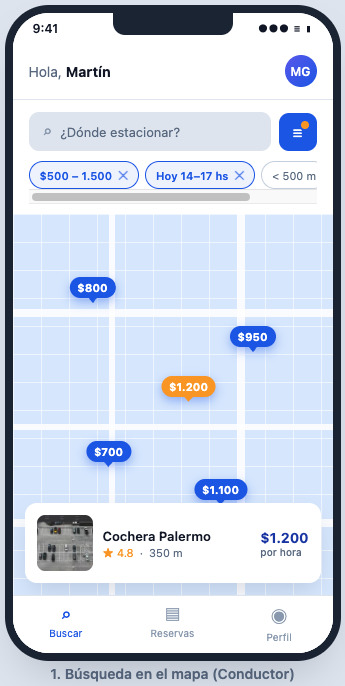
\includegraphics[width=0.45\textwidth]{img/mockup_busqueda.png}
    \caption{Búsqueda de cocheras en el mapa con filtros activos (conductor).}
    \label{fig:mockup_busqueda}
\end{figure}

\begin{figure}[H]
    \centering
    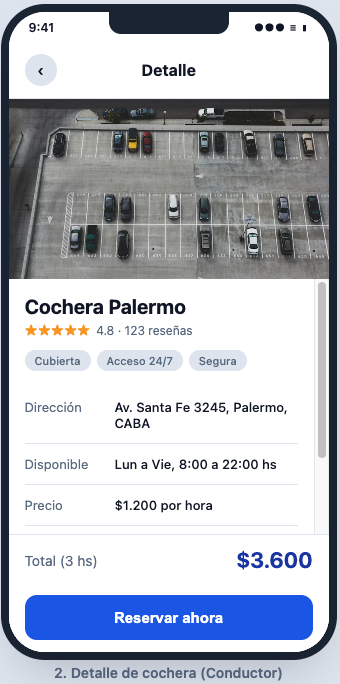
\includegraphics[width=0.45\textwidth]{img/mockup_detalle.png}
    \caption{Detalle de una cochera y selección de horario de reserva (conductor).}
    \label{fig:mockup_detalle}
\end{figure}

\begin{figure}[H]
    \centering
    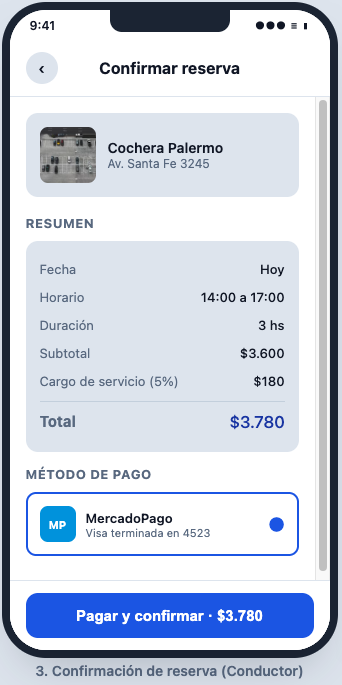
\includegraphics[width=0.45\textwidth]{img/mockup_reserva.png}
    \caption{Confirmación de reserva con resumen de costos y método de pago (conductor).}
    \label{fig:mockup_reserva}
\end{figure}

\begin{figure}[H]
    \centering
    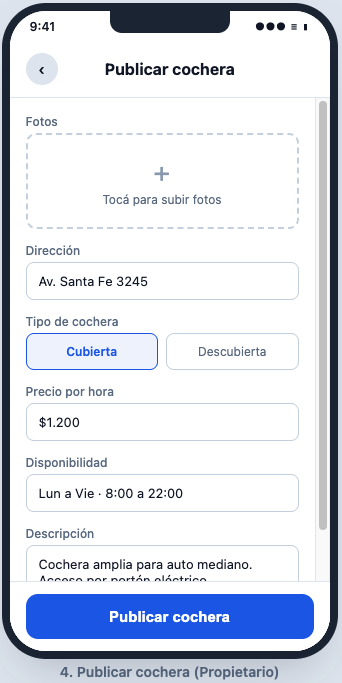
\includegraphics[width=0.45\textwidth]{img/mockup_publicar.png}
    \caption{Formulario de publicación de una cochera (propietario).}
    \label{fig:mockup_publicar}
\end{figure}

\begin{figure}[H]
    \centering
    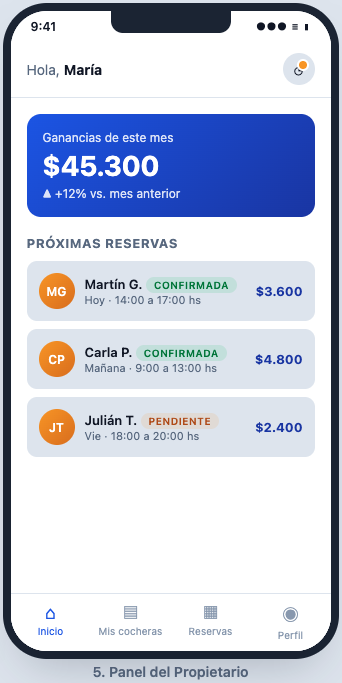
\includegraphics[width=0.45\textwidth]{img/mockup_propietario.png}
    \caption{Panel principal del propietario con ganancias y próximas reservas.}
    \label{fig:mockup_propietario}
\end{figure}

\section{Plan Económico y Modelo de Negocio}\label{sec:plan_economico}

Con el fin de validar la sostenibilidad financiera del proyecto, se desarrolló un modelo analítico segmentado en tres etapas de evolución: Corto plazo (MVP), mediano plazo y largo plazo. Los valores se expresan en dólares estadounidenses, tomando como tipo de cambio referencial 1 USD = 1.500 ARS.

\subsection{Estimación del mercado potencial (TAM, SAM, SOM)}

El orden de autos que circulan a diario en una ciudad del tamaño de Buenos Aires (CABA) es de aproximadamente 1,8 millones de vehículos diarios \autocite{superauto2024, aboy2025movilidad}, considerando tanto residentes como personas que ingresan desde el conurbano. Sin embargo, no todos representan clientes potenciales directos para ParkLink, ya que existen distintos perfiles de conductores y diferentes necesidades de estacionamiento.

Tomando como referencia patrones urbanos comunes en ciudades densamente pobladas, puede estimarse que entre un 10\% y un 15\% de los conductores diarios efectivamente necesitan buscar estacionamiento de manera activa. Esta estimación contempla:

\begin{itemize}
    \item Conductores que trabajan en oficinas y centros comerciales.
    \item Personas que realizan trámites médicos o administrativos.
    \item Usuarios ocasionales y visitantes de otras jurisdicciones.
    \item Personas que no cuentan con cochera fija en su destino.
\end{itemize}

En contrapartida, quedan excluidos perfiles con estacionamiento asegurado o sin necesidad de búsqueda activa:
\begin{itemize}
    \item Taxis, remises y vehículos de transporte público.
    \item Aplicaciones de movilidad de pasajeros (Uber, Cabify, Didi).
    \item Personas con cochera fija propia o alquilada mensualmente.
    \item Usuarios de parada muy breve (\textit{drop-off}).
\end{itemize}

Bajo esta hipótesis, el mercado objetivo potencial diario dentro de CABA se clasifica en tres escenarios:
\begin{itemize}
    \item \textbf{Escenario conservador (10\%):} 180.000 búsquedas diarias de estacionamiento.
    \item \textbf{Escenario medio (12\%):} 216.000 búsquedas diarias.
    \item \textbf{Escenario optimista (15\%):} 270.000 búsquedas diarias.
\end{itemize}

Naturalmente, ParkLink no captaría todo ese mercado desde el primer momento. La adopción real se desarrolla en una rampa progresiva a lo largo de varios años de operación, partiendo de niveles bajos durante la etapa de validación y creciendo a medida que se consolida la marca, se amplía la cobertura geográfica y se incrementa la oferta de cocheras disponibles.

\subsection{Rampa y curva de adopción por etapa}

Sobre la base del escenario medio de mercado potencial (216.000 búsquedas diarias), se proyecta el siguiente patrón de adopción:

\begin{itemize}
    \item \textbf{MVP (año 1):} Adopción del 0,025\% del mercado potencial (55 reservas diarias).
    \item \textbf{Mediano plazo (año 2):} Adopción del 0,28\% (600 reservas diarias).
    \item \textbf{Largo plazo (año 3 en adelante):} Adopción del 0,91\% (1.966 reservas diarias), consolidando CABA.
    \item \textbf{Largo plazo en el mejor caso:} Adopción del 1,5\% sobre el escenario optimista (4.050 reservas diarias).
\end{itemize}

La cantidad de reservas diarias proyectadas en cada etapa se resume en la Tabla~\ref{tab:adopcion}.

\begin{table}[H]
    \centering
    \caption{Reservas diarias proyectadas por etapa.}
    \vspace{0.2cm}
    \resizebox{\textwidth}{!}{%
    \begin{tabular}{l r r}
        \toprule
        \textbf{Etapa} & \textbf{\% de adopción} & \textbf{Reservas diarias} \\
        \midrule
        MVP (año 1) & 0,025\% & 55 \\
        Mediano plazo (año 2) & 0,28\% & 600 \\
        Largo plazo & 0,91\% & 1.966 \\
        Largo plazo (mejor caso) & 1,5\% & 4.050 \\
        \bottomrule
    \end{tabular}%
    }
    \label{tab:adopcion}
\end{table}

\subsection{Precios de referencia del mercado en CABA}

Los precios del estacionamiento privado en CABA no están regulados y varían según la zona, el horario y el tipo de vehículo. De acuerdo con los relevamientos de precios más recientes, una hora de estacionamiento en una cochera o playa de la ciudad se ubica entre \$6.000 y \$10.000 ARS, con un valor promedio de aproximadamente \$8.000 ARS, y puede alcanzar los \$20.000 ARS en las zonas y horarios de mayor demanda \autocite{iprofesional2026cocheras}. Para las estadías más extensas, el precio por hora disminuye: Una estadía diaria ronda los \$39.000 ARS, por debajo de lo que costaría una jornada completa a tarifa horaria, mientras que el alquiler mensual de una cochera varía entre \$100.000 y \$350.000 ARS según el barrio \autocite{iprofesional2026cocheras, lanacion2026cocheras}.

Tomando como referencia una reserva típica de estadía corta de dos horas y media, el ticket promedio por reserva se establece en \$20.000 ARS (USD 13,33).

\subsection{Estructura y modelo de ingresos}

El modelo de negocio de ParkLink es transaccional y cobra únicamente al conductor. Publicar una cochera es gratuito y el propietario recibe el 100\% del precio que fija para su espacio. La plataforma obtiene sus ingresos mediante un cargo de servicio del 8\% que se suma al valor de cada reserva concretada y que abona el conductor al momento del pago. De esta forma, ParkLink solo genera ingresos cuando se concreta una reserva, y el propietario no tiene ningún costo por formar parte de la plataforma.

La Tabla~\ref{tab:ingreso_por_reserva} muestra el ingreso que genera cada tipo de reserva.

\begin{table}[H]
    \centering
    \caption{Ingreso de la plataforma por tipo de reserva (cargo de servicio del 8\%).}
    \vspace{0.2cm}
    \small
    \renewcommand{\arraystretch}{1.3}
    \begin{tabular}{l r r r r}
        \toprule
        \textbf{Tipo de reserva} & \textbf{Recibe el propietario} & \textbf{Paga el conductor} & \multicolumn{2}{c}{\textbf{Ingreso de ParkLink}} \\
        \cmidrule(lr){4-5}
         & \textbf{(ARS)} & \textbf{(ARS)} & \textbf{ARS} & \textbf{USD} \\
        \midrule
        Estadía corta (2,5 h) & 20.000 & 21.600 & 1.600 & 1,07 \\
        Estadía diaria & 39.000 & 42.120 & 3.120 & 2,08 \\
        Alquiler mensual & 100.000--350.000 & 108.000--378.000 & 8.000--28.000 & 5,33--18,67 \\
        \bottomrule
    \end{tabular}
    \label{tab:ingreso_por_reserva}
\end{table}

Para las proyecciones se adoptó un criterio conservador: Todas las reservas se estiman con el ticket de la estadía corta, que es el de menor valor. Las reservas por día y por mes, que generan un ingreso mayor por operación, representan un potencial adicional que no se incluye en los cálculos.

\subsection{Estimación de ingresos y resultados financieros}

Multiplicando las reservas diarias proyectadas por el ingreso promedio por operación (USD 1,07), los ingresos diarios, mensuales y anuales esperados por etapa son los siguientes:

\begin{table}[H]
    \centering
    \caption{Ingresos proyectados por etapa (en USD).}
    \vspace{0.2cm}
    \resizebox{\textwidth}{!}{%
    \begin{tabular}{l r r r r}
        \toprule
        \textbf{Etapa} & \textbf{Reservas/día} & \textbf{Ingreso diario} & \textbf{Ingreso mensual} & \textbf{Ingreso anual} \\
        \midrule
        MVP (año 1)              & 55    & 58,67    & 1.760   & 21.120 \\
        Mediano plazo (año 2)    & 600   & 640,00   & 19.200  & 230.400 \\
        Largo plazo              & 1.966 & 2.097,07 & 62.912  & 754.944 \\
        Largo plazo (mejor caso) & 4.050 & 4.320,00 & 129.600 & 1.555.200 \\
        \bottomrule
    \end{tabular}%
    }
    \label{tab:ingresos_etapas}
\end{table}

\subsection{Estructura de costos, inversión y punto de equilibrio}

\subsubsection{Premisas operativas}

\begin{itemize}
    \item Vehículos circulantes diarios en CABA: Aproximadamente 1,8 millones de vehículos.
    \item Proporción de conductores que buscan estacionamiento de manera activa: 12\% en escenario medio.
    \item Valor promedio de una hora de cochera en CABA: \$8.000 ARS (rango de \$6.000 a \$10.000 ARS).
    \item Ticket promedio por reserva de estadía corta (2,5 horas): \$20.000 ARS (USD 13,33).
    \item Modelo de ingresos: Cargo de servicio del 8\% abonado por el conductor, equivalente a USD 1,07 por operación exitosa.
    \item Año operativo de 360 días (12 meses de 30 días) y tipo de cambio de referencia de 1 USD = 1.500 ARS.
\end{itemize}

\subsubsection{Gastos operativos por etapa}

La estructura de costos contempla sueldos escalonados de los cuatro fundadores, infraestructura tecnológica, marketing, gastos legales y soporte al usuario.

\begin{table}[H]
    \centering
    \caption{Gastos operativos mensuales y anuales estimados por etapa (en USD).}
    \vspace{0.2cm}
    \resizebox{\textwidth}{!}{%
    \begin{tabular}{l r r r r}
        \toprule
        \textbf{Rubro} & \textbf{MVP} & \textbf{Mediano} & \textbf{Largo plazo} & \textbf{Largo plazo (mejor caso)} \\
        \midrule
        Sueldos (4 fundadores)          & 6.000  & 8.000  & 10.000 & 10.000 \\
        Infraestructura tecnológica     & 25     & 300    & 600    & 900 \\
        Marketing y adquisición         & 300    & 1.200  & 1.500  & 2.500 \\
        Gastos legales y contables      & 200    & 400    & 500    & 500 \\
        Soporte al usuario              & 0      & 200    & 500    & 1.000 \\
        \midrule
        \textbf{Total mensual}          & \textbf{6.525}  & \textbf{10.100} & \textbf{13.100} & \textbf{14.900} \\
        \textbf{Total anual}            & \textbf{78.300} & \textbf{121.200}& \textbf{157.200}& \textbf{178.800} \\
        \bottomrule
    \end{tabular}%
    }
    \label{tab:gastos_operativos_etapas}
\end{table}

\subsubsection{Proyecciones financieras y rentabilidad}

La rampa de crecimiento contempla un lanzamiento focalizado en barrios de alta demanda durante el primer año, expansión zonal en el segundo año y consolidación a partir del tercer año.

\begin{table}[H]
    \centering
    \caption{Proyecciones financieras estimadas por etapa (en USD).}
    \vspace{0.2cm}
    \resizebox{\textwidth}{!}{%
    \begin{tabular}{l c r r r}
        \toprule
        \textbf{Etapa} & \textbf{Reservas diarias} & \textbf{Ingreso anual} & \textbf{Gastos operativos anuales} & \textbf{Resultado anual} \\
        \midrule
        MVP (año 1)               & 55    & 21.120    & 78.300  & -57.180 \\
        Mediano plazo (año 2)     & 600   & 230.400   & 121.200 & +109.200 \\
        Largo plazo               & 1.966 & 754.944   & 157.200 & +597.744 \\
        Largo plazo (mejor caso)  & 4.050 & 1.555.200 & 178.800 & +1.376.400 \\
        \bottomrule
    \end{tabular}%
    }
    \label{tab:resultados_etapas}
\end{table}

\paragraph{Inversión inicial requerida:}
El déficit operativo del primer año (USD 57.180) representa el capital mínimo necesario para sostener la operación durante la etapa de validación. De los USD 78.300 de gastos operativos anuales del MVP, USD 72.000 (el 92\%) corresponden al pago de salarios de los cuatro fundadores. Esto significa que la inversión inicial cubre fundamentalmente el costo del equipo durante la etapa previa al equilibrio: Sin remuneraciones, la operación cerraría con un superávit de USD 14.820 incluso en su primer año. Considerando un margen de contingencia del 20\%, la inversión inicial estimada asciende a aproximadamente USD 69.000.

\paragraph{Punto de equilibrio y rentabilidad a escala:}
En el segundo año la operación alcanza el punto de equilibrio y genera ganancias, con un resultado positivo de USD 109.200 que permite recuperar en ese mismo año la totalidad de la inversión inicial. En el escenario de largo plazo se proyecta una utilidad neta anual de aproximadamente USD 600.000, suficiente para sostener salarios competitivos de los cuatro fundadores, cubrir obligaciones impositivas, reinvertir en la operación y financiar la expansión a nuevas zonas.

\section{Impactos sociales y ambientales del proyecto}

Más allá de su viabilidad económica, ParkLink tiene el potencial de generar beneficios concretos sobre el entorno urbano, la calidad de vida de los ciudadanos y el medioambiente. Estos efectos, aunque difíciles de monetizar directamente, constituyen una parte fundamental de la propuesta de valor del proyecto.

\subsection*{Reducción de la congestión vehicular}

Una fracción significativa del tránsito urbano en ciudades densas no obedece a desplazamientos con destino definido, sino a vehículos circulando en búsqueda de estacionamiento. Estudios realizados en distintas ciudades del mundo estiman que entre el 30\% y el 40\% del tráfico en zonas céntricas corresponde a conductores buscando dónde estacionar \autocite{shoup2006, shoup2005}. En CABA, con aproximadamente 1,8 millones de vehículos circulando diariamente, incluso una mejora marginal en la eficiencia de este proceso tendría un impacto agregado considerable sobre la fluidez del tránsito.

Al permitir que el conductor reserve su lugar antes de salir, ParkLink elimina la circulación improductiva: el vehículo se desplaza directamente hacia el espacio confirmado, sin vueltas ni tiempos muertos. A escala, esto implica menos autos en movimiento sin destino claro, menor ocupación de arterias viales y una mejora tangible en los tiempos de traslado.

\subsection*{Disminución de emisiones contaminantes}

La circulación innecesaria en busca de estacionamiento no solo genera congestión; también implica consumo adicional de combustible y emisión de gases de efecto invernadero. Cada minuto de motor encendido sin avance productivo equivale a combustible quemado y dióxido de carbono liberado sin contrapartida de utilidad.

Si ParkLink logra evitar, en promedio, entre 10 y 15 minutos de búsqueda por reserva exitosa, el ahorro acumulado en emisiones a lo largo de miles de operaciones diarias resultaría cuantificable y significativo. En un contexto global donde las ciudades buscan reducir su huella de carbono y mejorar la calidad del aire, la optimización del estacionamiento urbano representa una palanca concreta de intervención.

\subsection*{Mejor aprovechamiento de la infraestructura existente}

Uno de los problemas identificados en el análisis es la subutilización de espacios privados que permanecen vacíos durante buena parte del día. ParkLink no propone construir nueva infraestructura, sino hacer visible y accesible la que ya existe. Esto se alinea con el principio de economía colaborativa: extraer valor de activos ociosos, reduciendo la presión sobre los recursos urbanos disponibles y postergando la necesidad de ampliar la oferta de estacionamiento público.

\subsection*{Beneficios sobre la calidad de vida}

La búsqueda de estacionamiento es una fuente frecuente de estrés, demoras y frustración para los conductores urbanos. La posibilidad de planificar el estacionamiento con anticipación reduce la incertidumbre del traslado, mejora la experiencia del conductor y libera tiempo que de otro modo se destinaría a circular sin rumbo. Este beneficio, aunque subjetivo, tiene impacto directo sobre el bienestar cotidiano de una porción relevante de la población activa.

Adicionalmente, para los propietarios de cocheras, ParkLink representa la posibilidad de generar un ingreso pasivo a partir de un bien inmueble subutilizado, mejorando su situación económica sin requerir esfuerzo operativo adicional.

\subsection*{Alineación con políticas de movilidad urbana sostenible}

Las tendencias actuales en planificación urbana priorizan la reducción del uso del automóvil privado y la mejora de la eficiencia del tránsito. Si bien ParkLink no desincentiva el uso del auto, sí contribuye a que cada viaje sea más eficiente, reduciendo la circulación innecesaria que deriva de la falta de información sobre disponibilidad. En este sentido, la plataforma es compatible con y complementaria a políticas de movilidad sostenible que buscan reducir la congestión y las emisiones sin prohibir el acceso vehicular.

\section{Metodología de Trabajo}
Para la gestión del ciclo de vida del desarrollo se adoptará un enfoque metodológico híbrido que combina prácticas de \textbf{Scrum} y \textbf{Kanban}, asegurando adaptabilidad ante cambios de requisitos e iteraciones rápidas sin perder la predictibilidad del alcance global.

\subsection{Definición de Roles}
\begin{itemize}
    \item \textbf{Equipo de Alumnos:} Responsables directos de la arquitectura, codificación, aseguramiento de la calidad (QA), descubrimiento de requisitos, mitigación de riesgos y documentación técnica.
    \item \textbf{Cuerpo de Tutores:} Actuarán como facilitadores y \textit{Stakeholders} clave, validando el incremento de valor al cierre de cada ciclo y asistiendo en la priorización del \textit{Product Backlog}.
\end{itemize}

\subsection{Dinámica de Trabajo y Gestión de Tiempos}
\begin{itemize}
    \item \textbf{Sprints Bisemanales:} Ciclos fijos de desarrollo orientados a la entrega de módulos potencialmente desplegables.
    \item \textbf{Sprint Planning y Estimación:} Planificación al inicio de cada sprint utilizando la técnica de \textit{Planning Poker} basada en la escala de Fibonacci para asignar puntos de historia de manera consensuada.
    \item \textbf{Review y Retrospectiva:} Reuniones al cierre de cada iteración para demostrar las funcionalidades ante los tutores, recibir feedback y refinar los procesos internos del equipo.
\end{itemize}
\section{Experimentación y/o validación}\label{sec:validacion}

La validación de ParkLink se abordó en dos planos complementarios. En el plano técnico, se verificó que el sistema funcionara correctamente y de forma confiable, mediante pruebas automatizadas, pruebas integradas de punta a punta y controles de calidad del código. En el plano de producto, se contrastó la propuesta con potenciales usuarios reales para confirmar que resolvía una necesidad concreta y para detectar las dudas y fricciones que podían frenar su adopción. Se completó además una validación legal de la operatoria de la plataforma.

\subsection{Estrategia de validación y responsables}

La estrategia de pruebas siguió el enfoque de la pirámide de pruebas: Una base amplia de pruebas unitarias automatizadas, que verifican cada regla de negocio de forma aislada; un nivel intermedio de pruebas de integración, que verifican la interacción de cada servicio con su base de datos y con los servicios de los que depende; y un nivel superior, más reducido, de pruebas de punta a punta, que recorren los flujos completos tal como los ejecuta un usuario.

Cada integrante fue responsable de escribir y mantener las pruebas de los componentes a su cargo. La definición de los casos de prueba de los flujos completos, la ejecución de las pruebas exploratorias y el seguimiento de los defectos detectados estuvieron a cargo de los responsables de aseguramiento de la calidad, Santiago Domínguez y Santiago Jorge Varga.

\subsection{Validación técnica automatizada}

Los servicios del sistema incorporaron pruebas automatizadas con el marco de pruebas correspondiente a cada lenguaje, descripto en la Sección~\ref{sec:herramientas}. La Tabla~\ref{tab:pruebas} resume la cantidad de archivos de prueba de cada componente al cierre del desarrollo.

\begin{table}[H]
\centering
\renewcommand{\arraystretch}{1.3}
\small
\begin{tabular}{l l r}
\toprule
\textbf{Componente} & \textbf{Marco de pruebas} & \textbf{Archivos de prueba} \\
\midrule
\textit{booking-service} & Paquete de pruebas de Go, \textit{testify}, \textit{gomock} & 72 \\
\textit{notifications-service} & \textit{pytest} & 17 \\
\textit{auth-service} & \textit{pytest} & 10 \\
\textit{mobile} & \textit{Jest} & 9 \\
\textit{parking-service} & \textit{Jest} & 7 \\
\textit{payment-service} & \textit{Jest}, \textit{supertest} & 7 \\
\textit{gateway} & \textit{pytest} & 6 \\
\midrule
\textbf{Total} & & \textbf{128} \\
\bottomrule
\end{tabular}
\caption{Archivos de pruebas automatizadas por componente.}
\label{tab:pruebas}
\end{table}

La distribución de las pruebas refleja dónde se concentra el riesgo del sistema: El servicio de reservas, que contiene la mayor parte de las reglas de negocio, reunió más de la mitad de los archivos de prueba. Entre los casos críticos que se verificaron de forma automatizada se encuentran los siguientes:

\begin{itemize}
    \item \textbf{Cálculo de disponibilidad:} La resta de las reservas activas sobre las franjas publicadas por el propietario, incluyendo bordes de horarios, cambios de día y la conversión entre la hora local y la hora universal.
    \item \textbf{Reservas concurrentes:} Que dos solicitudes simultáneas sobre el mismo lugar no puedan generar una sobre-reserva, y que la retención temporal del lugar expire correctamente si el pago no se completa.
    \item \textbf{Códigos de verificación:} La generación y validación de los códigos de ingreso y de egreso, y el cálculo del cargo por permanencia excedida.
    \item \textbf{Pagos:} La verificación de la firma de las notificaciones de Mercado Pago, la confirmación de la reserva asociada y los reintentos automáticos de los reembolsos.
    \item \textbf{Eventos y notificaciones:} Que un mismo evento recibido más de una vez no genere notificaciones duplicadas, y que los mensajes malformados no bloqueen el procesamiento del resto.
    \item \textbf{Puerta de enlace:} La validación de los tokens de acceso, el rechazo de solicitudes sin credenciales y la eliminación de los encabezados internos que un cliente externo intentara falsificar.
\end{itemize}

Estas pruebas se ejecutaron automáticamente ante cada cambio mediante el circuito de integración continua, junto con el análisis estático del código y la verificación de tipos, de modo que ningún cambio con errores detectables se incorporara a la rama principal.

\subsection{Pruebas integradas y de punta a punta}

Además de las pruebas de cada servicio, se validó el funcionamiento del sistema completo. Para ello se desarrolló un \textit{script} de prueba de punta a punta que, con todos los servicios en ejecución, recorre el flujo principal de la plataforma: Crea un propietario, publica una cochera con su horario y precio, crea un conductor, consulta la disponibilidad, genera una reserva y verifica que cada paso produzca el resultado esperado. Este \textit{script} permitió comprobar rápidamente, después de cada integración, que los servicios seguían funcionando correctamente en conjunto.

Las pruebas manuales se realizaron sobre los tres entornos de ejecución descriptos en la Sección~\ref{sec:dinamica}. En particular, la posibilidad de exponer el entorno a la red local y a internet permitió probar la aplicación desde teléfonos Android e iOS reales, verificando aspectos que un emulador no reproduce con fidelidad, como la recepción de notificaciones \textit{push}, el uso de la ubicación del dispositivo y la redirección al entorno de pago de Mercado Pago y su regreso a la aplicación. Los pagos se probaron en el entorno de pruebas de Mercado Pago, con usuarios compradores de prueba, sin movimiento de dinero real. Para estas pruebas se utilizó un generador de datos de demostración con cocheras distribuidas en distintos barrios de la Ciudad de Buenos Aires, que permitió evaluar la búsqueda en el mapa y la navegación en condiciones similares a las de uso real.

\subsection{Validación de mercado mediante encuesta}\label{sec:encuesta}

Para validar la propuesta con potenciales usuarios, el equipo realizó una encuesta difundida a través de la red social Instagram, dirigida a personas de distintos perfiles de la Ciudad de Buenos Aires. Se obtuvieron \textbf{180 respuestas}. La mayoría de quienes respondieron fueron conductores frecuentes, aunque también participó un grupo numeroso de personas con cocheras libres interesadas en aprovecharlas, lo que permitió relevar la visión de ambos lados del mercado.

\subsubsection{Aceptación de la propuesta}

La propuesta tuvo una aceptación alta. La posibilidad de salir de casa con el lugar ya reservado y pagado fue el aspecto mejor valorado, con calificaciones de 4 o 5 puntos sobre 5 en la gran mayoría de las respuestas. En cuanto a la frecuencia de uso, alrededor del 70\% de los encuestados indicó que usaría la aplicación de forma regular, con frecuencias que van desde algunas veces al mes hasta todos los días.

Entre los motivos para utilizar ParkLink, se destacaron tres:

\begin{itemize}
    \item \textbf{El precio:} Conocer el precio de antemano y que resulte más conveniente que el de una playa comercial fue el motivo principal. Los encuestados indicaron que estarían dispuestos a pagar entre \$4.000 y \$6.000 por hora.
    \item \textbf{La cercanía:} Estacionar lo más cerca posible del destino final fue otro de los motivos más votados.
    \item \textbf{El cuidado del vehículo:} Muchos encuestados prefieren dejar el auto en una cochera de barrio antes que en la calle, expuesto a rayones o robos.
\end{itemize}

\subsubsection{Fricciones detectadas y decisiones de producto}

La encuesta permitió identificar las principales dudas de cada lado del mercado. Del lado del conductor, el temor más mencionado fue llegar a la cochera y encontrarla ocupada porque el conductor del turno anterior no se había retirado; le siguieron las dudas sobre cómo ingresar a una cochera privada sin control remoto y la necesidad de confiar en que el espacio publicado existiera realmente. Del lado del propietario, la duda más repetida fue de índole legal, ya que muchos reglamentos de copropiedad no permiten el ingreso de vehículos de personas ajenas al edificio; también surgieron el deseo de obtener un ingreso sin tener que estar presente para abrir el portón y la preocupación por quién se hace cargo ante un eventual daño.

Cada una de estas fricciones se tradujo en una decisión concreta que se incorporó al producto, como resume la Tabla~\ref{tab:encuesta_decisiones}.

\begin{table}[H]
\centering
\renewcommand{\arraystretch}{1.35}
\small
\begin{tabularx}{\textwidth}{>{\raggedright\arraybackslash}p{4.6cm} >{\raggedright\arraybackslash}X}
\toprule
\textbf{Fricción detectada} & \textbf{Decisión implementada en ParkLink} \\
\midrule
Encontrar la cochera ocupada por el conductor anterior & Período de gracia de 15 minutos antes y después de cada reserva, que deja al menos 30 minutos libres entre reservas consecutivas, y verificación del ingreso y del egreso mediante códigos, con un cargo por permanencia excedida. \\
Cómo ingresar sin control remoto & Instrucciones de acceso privadas que el propietario carga en su publicación y que el conductor solo ve una vez aceptada su reserva. \\
Desconfianza sobre la existencia del espacio & Verificación obligatoria del correo y del teléfono de todos los usuarios, reseñas entre conductores y propietarios y revisión de cada nueva cochera por un administrador antes de publicarse. \\
Restricciones del reglamento de copropiedad & Carga obligatoria de documentación de respaldo (escritura, contrato de alquiler o expensas) revisada antes de la publicación, y declaración del propietario, en los Términos y Condiciones, de que tiene derecho a ofrecer la cochera. \\
Obtener ingresos sin estar presente & Reservas con confirmación instantánea, sin aprobación manual del propietario, cobro dentro de la aplicación y liquidación de las ganancias por parte de la plataforma. \\
Responsabilidad ante daños & Reglas de responsabilidad definidas en los Términos y Condiciones, denuncias y tickets de soporte asociados a cada reserva y mensajería directa entre las partes. \\
\bottomrule
\end{tabularx}
\caption{Fricciones relevadas en la encuesta y decisiones de producto derivadas.}
\label{tab:encuesta_decisiones}
\end{table}

Por último, el rango de precio que los conductores declararon estar dispuestos a pagar resultó inferior al valor promedio de mercado utilizado en el plan económico de la Sección~\ref{sec:plan_economico}. Este resultado confirma que el precio es el principal factor de decisión del conductor y refuerza la importancia de incorporar cocheras particulares que puedan competir con las playas comerciales, como se analizó en la Sección~\ref{sec:impactos}.

% TODO: Subsección de validación con el contacto externo (pendiente de recibir la información).

\subsection{Validación legal}\label{sec:validacion_legal}

Antes de que la plataforma pudiera ser utilizada por personas reales, se validó su operatoria desde el punto de vista legal. Se redactaron los Términos y Condiciones y la Política de Privacidad de ParkLink, publicados en el sitio oficial del proyecto. Los Términos regulan el funcionamiento de las reservas, los pagos, las cancelaciones, las liquidaciones a los propietarios y las responsabilidades de cada parte, exigen que los usuarios sean mayores de edad y que el propietario declare tener derecho a ofrecer la cochera publicada, y preservan los derechos que la Ley 24.240 de Defensa del Consumidor reconoce a los usuarios. La Política de Privacidad se elaboró conforme a la Ley 25.326 de Protección de los Datos Personales, detallando qué datos se recolectan, con qué finalidad, con quién se comparten, cuánto tiempo se conservan y cómo ejercer los derechos de acceso, rectificación y supresión. La aceptación de ambos documentos se incorporó como paso obligatorio del registro en la aplicación, que además permite consultarlos en todo momento y eliminar la cuenta propia.

\subsection{Resultados de la validación}

La validación técnica permitió llegar al cierre del desarrollo con los flujos críticos de la plataforma cubiertos por pruebas automatizadas que se ejecutan ante cada cambio, y con el recorrido completo de búsqueda, reserva, pago y notificación verificado sobre dispositivos reales. La validación de mercado confirmó el interés de ambos lados del mercado en la propuesta y, sobre todo, permitió anticipar las fricciones que podían frenar su adopción e incorporar al producto las decisiones necesarias para resolverlas antes de su lanzamiento. Finalmente, la validación legal dejó definidas las reglas que regulan la relación entre la plataforma, los conductores y los propietarios.

\section{Plan de Actividades}
El desarrollo se segmentará temporalmente respetando las fases típicas de un proyecto de ingeniería. El cronograma maestro contempla las siguientes macro-actividades distribuidas a lo largo del período lectivo:

\begin{enumerate}
    \item \textbf{Fase de Investigación y Requisitos:} Refinamiento del target de usuarios (conductores vs. rentadores) y definición de requisitos funcionales y no funcionales.
    \item \textbf{Fase de Diseño y Arquitectura:} Modelado de la base de datos (relacional/NoSQL), diseño de interfaces de usuario (\textit{Mockups}) y definición de contratos de API.
    \item \textbf{Fase de Desarrollo del MVP:} Implementación secuencial de los módulos de autenticación, mapeo cartográfico, lógica de reservas manuales e integración de pasarela de pagos.
    \item \textbf{Fase de Pruebas e Implementación:} Ejecución del plan de validación, corrección de defectos y despliegue inicial en entornos de pruebas controlados (\textit{Staging}).
    \item \textbf{Fase de Cierre y Documentación:} Redacción del informe final, preparación de minutas y confección del manual de despliegue técnico.
\end{enumerate}

\newpage
\printbibliography[title={Referencias}]

\end{document}